%% TCC - Monografia
%% Ci\^{e}ncia da Computa\c{c}\~{a}o - LCMAT - CCT - UENF, 2018
%% 

\chapter{Arquitetura microsserviços}\label{cap5}

\section{Criação do fluxo das arquiteturas}

Como todo projeto a ser desenvolvido, precisamos planejar e analisar todas as tecnologias, fluxos e informações sobre o que desejamos fazer. No desenvolvimento de software não é diferente, precisamos criar um fluxograma da arquitetura.

O planejamento da arquitetura baseada em microsserviços seguirá os mesmos passos já feito para a arquitetura em camadas. O fluxograma tem uma visão macro da comunicação entre os sistemas e na fase de implementação seguiremos o fluxograma e modificaremos ao longo do processo.

\subsubsection{Fluxograma da arquitetura baseada em microsserviços}

O projeto baseado nesse tipo de arquitetura segue a utilização de diversos serviços distintos que se comunicam entre si como pode ser verificar no fluxograma da \ref{fig:microservice-fluxograma}.

O projeto para nos dará dados estatísticos sobre o assédio moral ou sexual nas Universidade, cidades, estados e países, e também será uma aplicação colaborativa, onde não sabemos a quantidade de usuários que iremos atingir e quantos desenvolvedores irão colaborar com esse projeto, então, uma arquitetura baseada em microsserviços poderá ser uma escolha ótima escolha, haja visto que poderemos contar com diversas comunidades, seja em termos de desenvolvimento de novas funcionalidades com as funcionalidades que poderão ser feitas em qualquer tecnologias e também em termos de acesso por diversos departamentos ou instâncias da sociedade, como departamento de segurança, Universidades, empresas de seguro com o intuito de analisar os riscos sobre uma determinada apólice ou mesmo a população, tendo em vista que com informações reais a cobrança será muito mais bem fundamentada para cobrar os governantes. 

\begin{figure}[htbp]
\hypertarget{arquitetura}{%
\caption{UML mostrando o fluxo da arquitetura baseada em microsserviços}
\begin{center}
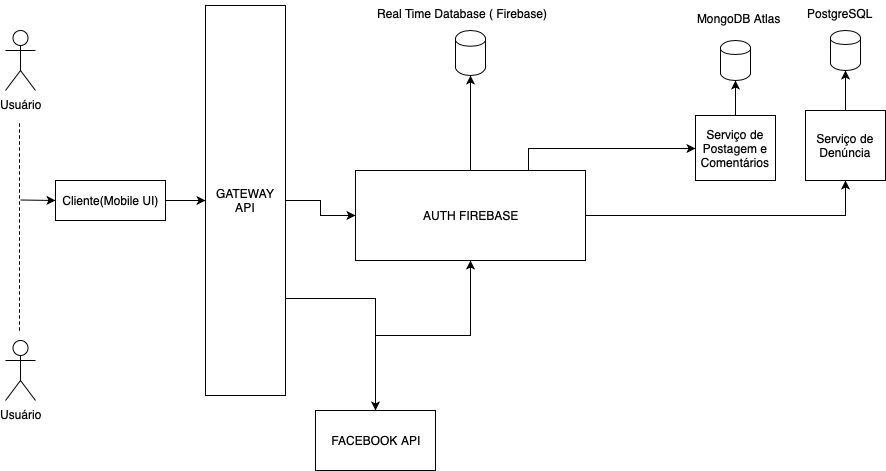
\includegraphics[width=15cm]{Monografia-FormatoLatex/Imagens/microservice-fluxograma.png}
\end{center}
}
\legend{Fonte: Criado pelo autor no site draw.io}
\label{microservice-fluxograma}
\end{figure}

\subsection{Cliente (Mobile UI)}
  
  A arquitetura proposta precisa de uma interface de entrada de dados para iteração dos usuários. O usuário executa uma ação no cliente que no nosso caso é um aplicativo mobile e inicia o fluxo que vai para a parte do API Gateway.
  
\subsection{API Gateway}

  Quando se desenvolve um sistema baseado na arquitetura de microsserviços alguns problemas aparecem, como por exemplo, precisaríamos fazer o cliente, que poderia ser um outro sistema, aplicativo, página web ou qualquer outra forma de consumir uma API conhecer diversos endpoints e versões das APIs e não seria uma forma transparente como um monolítico é, então criamos um microsserviços para cuidar dessa parte de redirecionar, verificar a autorização e a permissão do usuário. Imagino um cenário de uma arquitetura baseada em microsserviços com uns 20 sistemas, como você faria para fazer a autorização e a autenticação dos seus usuários? seria bem complexo, correto? Porém com um único ponto de entrada você torna esse processo mais simples.

\subsection{Serviço de Postagem e Comentários}

Os microsserviços são totalmente isolados e por isso cada parte tem o seu próprio banco de dados. Como podemos analisar na figura \ref{fig:microservice-fluxograma}. O serviço de postagem e comentários tem o contexto de cadastrar, excluir, deletar ou atualizar um comentário ou uma postagem. Como a postagem está totalmente acoplada aos comentários que foram feitas nele. Por exemplo, uma postagem que vamos dar o nome de \textbf{postagem1} está ligado aos comentários que vamos chamar de \textbf{comentario}, \textbf{comentario2} e \textbf{comentario}. Nesse contexto não faria sentido termos dois serviços um postagem e o outro para comentários, visto que eles fazem parte de um contexto definido.

\subsection{Serviço de Denúncia}

O serviço para denúncias também faz parte de um contexto próprio com seu banco de dados também próprio. As informações de cadastro e acompanhamento da denuncia será feita totalmente por esse serviço. O usuário poderá em um passo a passo fazer a denúncia do ocorrido e a plataforma se encarregará de enviar essas informações para um órgão competente, por exemplo nas Universidades.


\section{Implementação da Arquitetura}

O código da implementação dos microsserviços seguem abaixo:


\begin{enumerate}
    \item API Users - https://github.com/rodolfopeixoto/obsidium-users-api
    \item API Gateway - https://github.com/rodolfopeixoto/obsidium-gateway-api
    \item Interface Mobile - https://github.com/amog-oliveira/obsidium/tree/develop
    \item PostIt - https://github.com/rodolfopeixoto/obsidium-postit
\end{enumerate}

\subsection{Cliente (MOBILE UI) }

 O cliente foi desenvolvido em React Native como já informado no capítulo 2, é uma tecnologia muito utilizada para se criar aplicativos nativos com uma maior produtividade de reutilização de código para duas ou até três plataformas distintas, como por exemplo Web, IOS e Android.

\subsection{API Gateway}

A API Gateway foi desenvolvida em NodeJS com Express. A API Gateway é responsável por fazer o redirecionamento paras as rotas corretas dos microsserviços, entretanto, antes da comunicação entre ela e outros serviços, é feita uma verificação de autenticação e a autorização, onde há uma comunicação com um outro serviço especializado em usuários e autenticação e autorização de forma transparente.

\subsubsection{Serviço de usuário (Firebase e API Facebook) }

O Firebase tem um importante papel no nosso sistema, pois ele nos da um sistema de autorização e autenticação pronto e um banco de dados para armazenar essas informações. Com ele podemos verificar se usuário através de sua interface pode acessar determinado recurso ou não.

A API do Facebook tem o papel de facilitar a vida dos usuários que querem acessar o sistema rapidamente, sem perder tempo com cadastros longos ou com senhas que se perdem ao longo do tempo.

\subsection{ Serviço de Postagem e Comentários }

O serviço de postagem e comentários foi desenvolvido também em NodeJS e Express, porém o banco de dados utilizado é o banco MongoDB Atlas. O sistema utiliza um banco de dados NoSQL e remoto, pois o banco de dados Atlas é um cloud com uma interface de fácil configuração e implementação, com o banco de dados remoto, não precisamos nos preocupar com a infra-estrutura mantida. 

\subsection{ Serviço de Denúncia }

O sistema de serviço de denúncias foi desenvolvido em Ruby on Rails com PostgreSQl e ambos containerizados e hospedados no heroku. É uma API relativamente simples que cadastra as denúncias e retorna as mesmas.
